\documentclass[aspectratio=169]{beamer}
\usetheme{metropolis}
\usecolortheme{default}

% Packages
\usepackage{graphicx}
\usepackage{tikz}
\usetikzlibrary{positioning}
\usepackage{booktabs}
\usepackage{listings}
\usepackage{xcolor}
\usepackage{amssymb}

% Colors
\definecolor{criticalred}{RGB}{220,53,69}
\definecolor{highorange}{RGB}{253,126,20}
\definecolor{mediumyellow}{RGB}{255,193,7}
\definecolor{lowgreen}{RGB}{40,167,69}
\definecolor{codeblue}{RGB}{0,123,255}

% Custom commands
\newcommand{\feature}[1]{\textcolor{codeblue}{$\checkmark$} \textbf{#1}}
\newcommand{\metric}[2]{\textbf{#1:} #2}
\newcommand{\cmark}{\textcolor{lowgreen}{$\checkmark$}}
\newcommand{\xmark}{\textcolor{criticalred}{$\times$}}

% Title page information
\title{Automated Phishing Email Detection System}
\subtitle{Prototype Threat Intelligence \& Risk Assessment Tool}
\author{Aser Osama - Saif Ismail - Omar Ayman}
\date{University of Science and Technology Zewail City}
\institute{October 2025}

\begin{document}

% ============================================================================
% TITLE SLIDE
% ============================================================================
\begin{frame}[plain]
\vspace*{-0.7cm}
\titlepage
\vspace*{-0.7cm}
\begin{center}
\scriptsize{A Research Prototype for Automated Phishing Detection}
\end{center}
\end{frame}

% ============================================================================
% TABLE OF CONTENTS
% ============================================================================
\begin{frame}{Presentation Overview}
\vspace{0.6cm}
\small
\tableofcontents
\vfill
\end{frame}

% ============================================================================
% SECTION 1: THE PROBLEM
% ============================================================================
\section{The Problem: Phishing Email Threats}

\begin{frame}{Email Security: A Critical Challenge}
\begin{columns}[T]
\column{0.5\textwidth}
\small
\textbf{The Threat Landscape:}
\begin{itemize}
    \item Over \textbf{255 million} phishing attacks in 2022
    \item Phishing is most common initial access
    \item Avg phishing site lifetime: \textbf{4-8 hours}
    \item Traditional detection too slow (24-72h)
\end{itemize}

\vspace{0.3cm}
\textbf{Current Challenges:}
\begin{itemize}
    \item Manual review doesn't scale
    \item Spam filters miss attacks
    \item Threat feeds lack context
    \item No unified risk assessment
\end{itemize}

\column{0.5\textwidth}
\small
\textbf{Our Approach:}
\begin{itemize}
    \item \cmark\ Aggregate threat feeds
    \item \cmark\ Enrich with technical context
    \item \cmark\ Automated risk scoring (0-100)
    \item \cmark\ Real-time email monitoring
    \item \cmark\ Visual dashboard interface
\end{itemize}

\vspace{0.1cm}
\begin{block}{Project Goal}
\scriptsize
\textbf{Open-source} prototype combining threat intel, enrichment, and risk scoring.
\end{block}
\end{columns}
\end{frame}

\begin{frame}{Why This Project?}
\vspace{-0.2cm}
\scriptsize
\textbf{Research Gap:} No open-source solution combines multi-feed aggregation, automated enrichment, risk prioritization, and deployable system.

\vspace{0.1cm}
\textbf{Existing Solutions:}

\begin{center}
\scriptsize
\begin{tabular}{lcc}
\toprule
\textbf{Type} & \textbf{Strengths} & \textbf{Limitations} \\
\midrule
Public Feeds & Free, high-volume & No enrichment \\
Commercial TIP & Comprehensive & Expensive \\
Email Gateways & Inline protection & Proprietary \\
\bottomrule
\end{tabular}
\end{center}

\vspace{0.1cm}
\begin{alertblock}{Our Contribution}
\scriptsize
Free, customizable prototype with automated enrichment and risk scoring
\end{alertblock}
\end{frame}

% ============================================================================
% SECTION 2: THE SOLUTION
% ============================================================================
\section{Our Solution: Automated Detection System}

\begin{frame}{System Overview}
\vspace*{-0.3cm}
\begin{center}
\small{\textbf{Phishing Email Detector Prototype}}

\vspace{0.1cm}
\scriptsize{Threat Intelligence + Risk Scoring + Email Monitoring}
\end{center}

\vspace{0.1cm}
\begin{columns}[T]
\column{0.33\textwidth}
\begin{block}{1. Aggregate}
\begin{center}
\small{$\bigstar$}
\end{center}
\scriptsize
3 threat feeds
\end{block}

\column{0.33\textwidth}
\begin{block}{2. Enrich}
\begin{center}
\small{$\blacktriangledown$}
\end{center}
\scriptsize
41 data points
\end{block}

\column{0.33\textwidth}
\begin{block}{3. Analyze}
\begin{center}
\small{$\bigodot$}
\end{center}
\scriptsize
Risk scores (0-100)
\end{block}
\end{columns}

\vspace{0.1cm}
\scriptsize
\textbf{DB:} 55K URLs | \textbf{Fields:} 41 | \textbf{Time:} 5-10 sec/email
\end{frame}

\begin{frame}{System Architecture}
\begin{center}
\scalebox{0.65}{
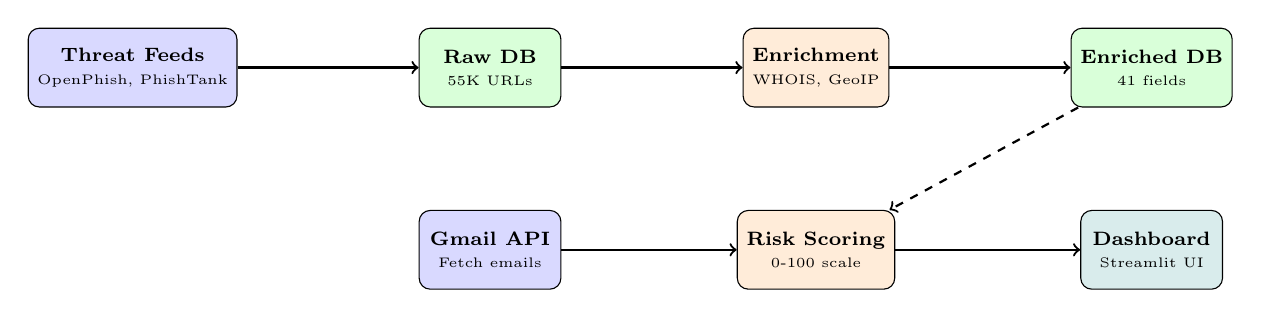
\begin{tikzpicture}[
    node distance=2.3cm,
    box/.style={draw, rectangle, rounded corners, minimum width=1.8cm, minimum height=1cm, align=center, font=\scriptsize},
    feed/.style={box, fill=blue!15},
    db/.style={box, fill=green!15},
    process/.style={box, fill=orange!15},
    ui/.style={box, fill=teal!15}
]

% Top row
\node[feed] (feeds) {\textbf{Threat Feeds}\\\tiny OpenPhish, PhishTank};
\node[db, right=of feeds] (rawdb) {\textbf{Raw DB}\\\tiny 55K URLs};
\node[process, right=of rawdb] (enrich) {\textbf{Enrichment}\\\tiny WHOIS, GeoIP};
\node[db, right=of enrich] (enrichdb) {\textbf{Enriched DB}\\\tiny 41 fields};

% Bottom row
\node[feed, below=1.3cm of rawdb] (gmail) {\textbf{Gmail API}\\\tiny Fetch emails};
\node[process, below=1.3cm of enrich] (scoring) {\textbf{Risk Scoring}\\\tiny 0-100 scale};
\node[ui, below=1.3cm of enrichdb] (dash) {\textbf{Dashboard}\\\tiny Streamlit UI};

% Arrows
\draw[->, thick] (feeds) -- (rawdb);
\draw[->, thick] (rawdb) -- (enrich);
\draw[->, thick] (enrich) -- (enrichdb);
\draw[->, thick] (gmail) -- (scoring);
\draw[->, thick] (scoring) -- (dash);
\draw[->, thick, dashed] (enrichdb) -- (scoring);
\end{tikzpicture}
}
\end{center}

\vspace{0.15cm}
\small
\textbf{Stack:} Python 3.11+, SQLite, FastAPI, Streamlit
\end{frame}

\begin{frame}{Where We Get Threat Data}
\small
\begin{columns}[T]
\column{0.5\textwidth}
\textbf{3 Public Threat Feeds:}
\begin{itemize}
    \item \textbf{OpenPhish:} 1,200 URLs
    \begin{itemize}
        \item \scriptsize Free, hourly updates
        \item \scriptsize Recently confirmed
    \end{itemize}
    \item \textbf{PhishTank:} 51,825 URLs
    \begin{itemize}
        \item \scriptsize Community-reported
        \item \scriptsize Brand targeting info
    \end{itemize}
    \item \textbf{URLhaus:} 2,317 URLs
    \begin{itemize}
        \scriptsize \item Malware sites
        \scriptsize \item File information
    \end{itemize}
\end{itemize}

\vspace{0.2cm}
\textbf{Total:} \textasciitilde55K URLs

\column{0.5\textwidth}
\textbf{41 Data Points Collected:}
\begin{itemize}
    \item \textbf{Network:} IP, hosting provider
    \item \textbf{Location:} Country, city
    \item \textbf{Security:} SSL certificate
    \item \textbf{Domain:} Registration info
    \item \textbf{DNS:} Name servers
    \item \textbf{Website:} Online status, title
    \item \textbf{Classification:} Target brand
\end{itemize}

\vspace{0.2cm}
\scriptsize
\textbf{Note:} Only 31\% have full WHOIS data
\end{columns}
\end{frame}

% ============================================================================
% SECTION 3: RISK SCORING
% ============================================================================
\section{Risk Scoring: How We Assess Threats}

\begin{frame}{Risk Scoring: How We Calculate 0-100 Score}
\small
\textbf{5 Factors Combined:}

\vspace{0.2cm}
\begin{enumerate}
    \item \textbf{\textcolor{criticalred}{Site online?}} (0-35 pts)
    \begin{itemize}
        \scriptsize
        \item Accessible: 35 pts; Offline: 10-20 pts
        \item \textit{Why:} Active sites more dangerous
    \end{itemize}
    
    \item \textbf{\textcolor{highorange}{Recently reported?}} (0-25 pts)
    \begin{itemize}
        \scriptsize
        \item Last 3 days: 25 pts; Last week: 20 pts; >30d: 5 pts
        \item \textit{Why:} Recent threats more active
    \end{itemize}
    
    \item \textbf{\textcolor{mediumyellow}{Domain age?}} (0-20 pts)
    \begin{itemize}
        \scriptsize
        \item <7 days: 20 pts; <30 days: 15 pts; >90d: 5 pts
        \item \textit{Why:} New domains suspicious
    \end{itemize}
\end{enumerate}
\end{frame}

\begin{frame}{Risk Scoring (Continued)}
\small
\begin{enumerate}
    \setcounter{enumi}{3}
    
    \item \textbf{\textcolor{codeblue}{Domain type?}} (0-10 pts)
    \begin{itemize}
        \scriptsize
        \item High-risk TLDs (.zip, .click, .xyz): 10 pts
        \item Free hosting (github.io, pages.dev): 10 pts
        \item Common (.com, .net, .org): 5 pts
        \item \textit{Why:} Cheap domains favored by attackers
    \end{itemize}
    
    \item \textbf{\textcolor{lowgreen}{Suspicious words?}} (0-10 pts)
    \begin{itemize}
        \scriptsize
        \item Has "login", "verify", "secure", etc: 10 pts
        \item No suspicious words: 0 pts
        \item \textit{Why:} Phishing uses trust words
    \end{itemize}
\end{enumerate}

\vspace{0.3cm}
\textbf{Final Score = Sum of all 5 factors (0-100)}

\vspace{0.2cm}
\begin{block}{Risk Levels}
\small
\textcolor{criticalred}{\textbf{85-100 Critical}} \quad
\textcolor{highorange}{\textbf{70-84 High}} \quad
\textcolor{mediumyellow}{\textbf{50-69 Medium}} \quad
\textcolor{lowgreen}{\textbf{0-49 Low}}
\end{block}
\end{frame}

\begin{frame}{Example: High-Risk URL Scoring}
\small
\begin{exampleblock}{Scenario: Suspicious URL Detected}
\scriptsize
\textbf{URL:} https://secure-login-microsoft.zip/verify
\end{exampleblock}

\vspace{0.2cm}
\textbf{Scoring Calculation:}
\begin{center}
\scriptsize
\begin{tabular}{lccc}
\toprule
\textbf{Factor} & \textbf{Points} & \textbf{Data} & \textbf{Logic} \\
\midrule
Liveness & 35 & HTTP 200 & Online \\
Recency & 25 & Today & $\leq$ 3 days \\
Domain Age & 20 & 2 days & $\leq$ 7 days \\
TLD & 10 & .zip & High-risk \\
Keywords & 10 & verify, login & Suspicious \\
\midrule
\textbf{Total} & \textbf{100} & & \textcolor{criticalred}{\textbf{CRITICAL}} \\
\bottomrule
\end{tabular}
\end{center}

\vspace{0.2cm}
\textbf{Legitimate Site (github.com):}
\begin{center}
\scriptsize
\begin{tabular}{lcl}
\toprule
Liveness: 35 & Domain Age: 5 (2008) & TLD: 5 (.com) \\
Recency: 5 (>30d) & Keywords: 0 & \textbf{Total: 50} \\
\bottomrule
\end{tabular}
\textcolor{mediumyellow}{\textbf{MEDIUM}} (acceptable)
\end{center}
\end{frame}

% ============================================================================
% SECTION 4: THE TECHNOLOGY
% ============================================================================
\section{Technology \& Architecture}

\begin{frame}{Email Monitoring Flow}
\vspace*{-1.0cm}
\begin{center}
\scalebox{0.37}{
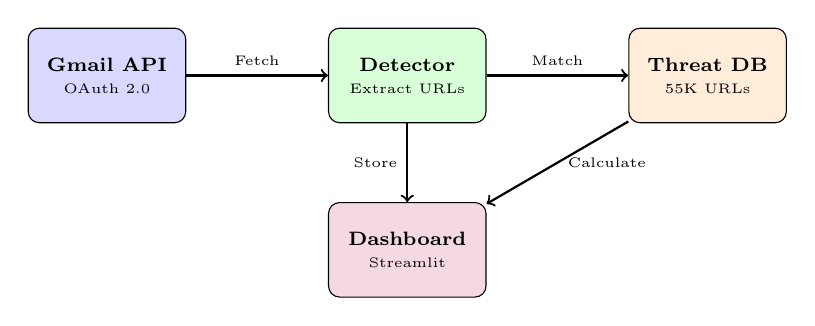
\begin{tikzpicture}[
    node distance=1.8cm,
    box/.style={draw, rectangle, rounded corners, minimum width=2cm, minimum height=1.2cm, align=center, font=\scriptsize},
    api/.style={box, fill=blue!15},
    process/.style={box, fill=green!15},
    data/.style={box, fill=orange!15},
    ui/.style={box, fill=purple!15}
]

% Nodes
\node[api] (gmail) {\textbf{Gmail API}\\\tiny OAuth 2.0};
\node[process, right=of gmail] (detector) {\textbf{Detector}\\\tiny Extract URLs};
\node[data, right=of detector] (db) {\textbf{Threat DB}\\\tiny 55K URLs};
\node[ui, below=1.0cm of detector] (dashboard) {\textbf{Dashboard}\\\tiny Streamlit};

% Arrows
\draw[->, thick] (gmail) -- node[above, font=\tiny] {Fetch} (detector);
\draw[->, thick] (detector) -- node[above, font=\tiny] {Match} (db);
\draw[->, thick] (db) -- node[right, font=\tiny] {Calculate} (dashboard);
\draw[->, thick] (detector) -- node[left, font=\tiny] {Store} (dashboard);
\end{tikzpicture}
}
\end{center}
\vspace{-0.5cm}
\tiny
\textbf{Processing:} 5-10 sec/email | \textbf{Interval:} 5 min
\end{frame}

\begin{frame}{Technology Stack}
\scriptsize
\begin{columns}[T]
\column{0.5\textwidth}
\textbf{Programming:}
\begin{itemize}
    \item \textbf{Python 3.11+}: FastAPI, Streamlit
    \item \textbf{SQLite}: 2 DBs (raw + enriched)
    \item \textbf{Gmail API}: Read-only OAuth
\end{itemize}

\vspace{0.15cm}
\textbf{Deployment:}
\begin{itemize}
    \item One command, Docker, Cross-platform
\end{itemize}

\column{0.5\textwidth}
\textbf{External Data:}
\begin{itemize}
    \item \textbf{Threat Intel}: PhishTank, URLhaus, OpenPhish
    \item \textbf{Enrichment}: WHOIS, GeoIP, DNS, HTTP
\end{itemize}

\vspace{0.15cm}
\textbf{Export:}
\begin{itemize}
    \item STIX 2.1, CSV, JSON API
\end{itemize}
\end{columns}

\vspace{0.15cm}
\begin{center}
\scriptsize
\textbf{Open Source on GitHub}
\end{center}
\end{frame}

% ============================================================================
% SECTION 5: THE DASHBOARD
% ============================================================================
\section{The Dashboard: Your Command Center}

\begin{frame}{Dashboard Interface (Streamlit)}
\textbf{5 Main Tabs:}

\begin{enumerate}
    \item \textbf{Email Monitoring}
    \item \textbf{Threat Overview}
    \item \textbf{Analytics}
    \item \textbf{Data Explorer}
    \item \textbf{Search}
\end{enumerate}
\end{frame}

\begin{frame}{Dashboard Tab Details}
\begin{itemize}
    \item \textbf{Email Monitoring:} Metrics, risk charts, timeline, filterable list
    \item \textbf{Threat Overview:} Statistics, geographic maps
    \item \textbf{Analytics:} ASN/TLD analysis
    \item \textbf{Data Explorer:} Browse 55K threats
    \item \textbf{Search:} URL/domain/IP lookup
\end{itemize}
\end{frame}

\begin{frame}{Dashboard: Top Metrics}
\begin{center}
\small
\begin{tabular}{ll}
\toprule
\textbf{Metric} & \textbf{Description} \\
\midrule
Total Emails & All in DB + 24h count \\
Critical Risk & Score $\geq$ 85 \\
High Risk & Score 70-84 \\
Avg Risk Score & Average \\
Threat Matches & External feed URLs \\
\bottomrule
\end{tabular}
\end{center}
\end{frame}

\begin{frame}{Dashboard: Email List Features}
\small
\textbf{Filters \& Display:}
\begin{itemize}
    \item Filter: Risk threshold slider
    \item Show: 25/50/100/200 emails
    \item Sort: By risk score or date
\end{itemize}

\vspace{0.2cm}
\textbf{Risk Levels:}
\begin{itemize}
    \item \textcolor{criticalred}{CRITICAL (85-100)}
    \item \textcolor{highorange}{HIGH (70-84)}
    \item \textcolor{mediumyellow}{MEDIUM (50-69)}
    \item \textcolor{lowgreen}{LOW (0-49)}
\end{itemize}
\end{frame}

% ============================================================================
% SECTION 6: DEPLOYMENT
% ============================================================================
\section{Deployment \& Usage}

\begin{frame}{Getting Started: One-Time Test}
\small
\textbf{Quick Start:}

\begin{block}{}
\texttt{\$ python run.py demo --once}
\end{block}

\vspace{0.2cm}
\textbf{Auto-setup steps:}
\begin{enumerate}
    \item Creates database schemas
    \item Downloads 55K threat URLs
    \item Quick enrichment (500 URLs)
    \item Gmail OAuth authentication
    \item Fetches 5 emails \& launches dashboard
\end{enumerate}

\vspace{0.2cm}
\textbf{Time:} 15-20 minutes (first run)
\end{frame}

\begin{frame}{Continuous Monitoring}
\small
\begin{block}{}
\texttt{\$ python run.py demo}
\end{block}

\vspace{0.2cm}
\textbf{Settings:}
\begin{itemize}
    \item Interval: 300 sec (5 min) - configurable
    \item Count: 5 emails per fetch - configurable
    \item Example: \texttt{--interval 60 --count 10}
\end{itemize}
\end{frame}

\begin{frame}{System Requirements}
\small
\textbf{Requirements:}
\begin{itemize}
    \item Python 3.11+
    \item 4-8 GB RAM
    \item 2 GB storage
    \item Linux, Mac, or Windows
\end{itemize}
\end{frame}

\begin{frame}{Performance \& Limitations}
\small
\textbf{Performance:}
\begin{itemize}
    \item Email analysis: 5-10 seconds
    \item Threat lookup: Instant
\end{itemize}

\vspace{0.2cm}
\textbf{Limitations:}
\begin{itemize}
    \item Tested with <1,000 emails
    \item WHOIS rate limited
    \item Larger scale needs DB upgrade
\end{itemize}
\end{frame}

% ============================================================================
% SECTION 7: EXAMPLE WALKTHROUGH
% ============================================================================
\section{Real Example: Threat Detection in Action}

\begin{frame}{Example: Phishing Email Detection}
\begin{block}{Email Received}
\textbf{From:} security-alert@paypal-verify.com\\
\textbf{Subject:} "Account Suspended"\\
\textbf{Content:} "Click: https://paypal-secure.xyz/login"
\end{block}
\end{frame}

\begin{frame}{Analysis Process - Step 1}
\textbf{URL Extraction:}

https://paypal-secure.xyz/login

\vspace{0.3cm}
\textbf{Threat Database Check:}
\begin{itemize}
    \item \xmark\ NOT found in PhishTank
    \item \xmark\ NOT found in URLhaus
    \item \cmark\ URL is new - needs risk calculation
\end{itemize}
\end{frame}

\begin{frame}{Analysis Process - Step 2}
\textbf{Risk Scoring Calculation:}
\begin{itemize}
    \item Liveness: 35 pts (site is online)
    \item Recency: 25 pts (domain seen today)
    \item Domain Age: 20 pts (created 3 days ago)
    \item TLD: 10 pts (.xyz = suspicious)
    \item Keywords: 10 pts ("paypal", "secure", "login")
\end{itemize}

\vspace{0.3cm}
\begin{alertblock}{Result}
\textbf{Total: 100/100 - CRITICAL RISK}
\end{alertblock}
\end{frame}

\begin{frame}{Dashboard Example: Email Details View}
\small
\textbf{What You See When You Click An Email:}

\vspace{0.2cm}
\begin{center}
\scriptsize
\fbox{\begin{minipage}{0.9\textwidth}
\small
\textbf{Email Monitoring Dashboard - Email Details}

\vspace{0.1cm}
\scriptsize
\textbf{Email Info:}
\begin{itemize}
    \item \textbf{From:} sender@example.com | \textbf{Subject:} "Check this link"
    \item \textbf{Risk:} \textcolor{criticalred}{\textbf{95/100}} | \textbf{URLs:} 1 | \textbf{Threats:} 0
\end{itemize}

\vspace{0.05cm}
\textbf{URLs Found:}

\scriptsize
\begin{tabular}{ll}
\toprule
\textbf{Risk} & \textbf{URL} \\
\midrule
\textcolor{criticalred}{95} & suspicious.zip/verify \\
\bottomrule
\end{tabular}

\vspace{0.05cm}
\textbf{Enrichment Data:}
\begin{itemize}
    \item \scriptsize Domain: suspicious.zip | TLD: .zip | IP: 93.184.216.34
    \item \scriptsize Country: US | ASN: AS15133 | Created: 2 days ago
    \item \scriptsize SSL: Yes | HTTP: 200 (online)
\end{itemize}
\end{minipage}}
\end{center}
\end{frame}

\begin{frame}{Email List View in Dashboard}
\vspace{-0.4cm}
\small
\textbf{Main Email Monitoring Tab:}

\vspace{0.0cm}
\begin{center}
\scriptsize
\begin{tabular}{lllcc}
\toprule
\textbf{Risk} & \textbf{From} & \textbf{Subject} & \textbf{URLs} & \textbf{Threats} \\
\midrule
\textcolor{criticalred}{100} & phish@bad.com & Verify Account & 1 & 1 \\
\textcolor{criticalred}{95} & spam@evil.zip & Click Here & 1 & 0 \\
\textcolor{highorange}{75} & ads@promo.xyz & Special Offer & 3 & 0 \\
\textcolor{mediumyellow}{55} & news@site.com & Newsletter & 5 & 0 \\
\textcolor{lowgreen}{45} & github.com & PR Review & 2 & 0 \\
\bottomrule
\end{tabular}
\end{center}

\vspace{0.1cm}
\scriptsize
\textbf{Features:} Filter ($\geq$70), Sort (risk/date), Limit (25/50/100/200), Click for details

\textbf{Threat Badge:} URLs matching external feeds
\end{frame}

% ============================================================================
% SECTION 8: LIMITATIONS & EVALUATION
% ============================================================================
\section{Limitations \& Evaluation}

\begin{frame}{Current Limitations}
\vspace*{-0.3cm}
\scriptsize
\textbf{1. WHOIS Coverage (31\%):} Privacy protection limits domain age data; using alternative signals

\vspace{0.1cm}
\textbf{2. Gmail-Only:} OAuth 2.0 only; no Exchange/Office 365; IMAP/SMTP planned

\vspace{0.1cm}
\textbf{3. No Content Analysis:} Metadata focus only; visual phishing not detected
\end{frame}

\begin{frame}{Performance \& Accuracy}
\small
\textbf{Database Statistics:}
\begin{itemize}
    \scriptsize
    \item \textbf{Total:} 55,225 unique URLs
    \item \textbf{OpenPhish:} 1,200 | \textbf{PhishTank:} 51,825 | \textbf{URLhaus:} 2,317
    \item \textbf{Enrichment:} 41 fields per URL
\end{itemize}

\vspace{0.2cm}
\textbf{Scoring Accuracy:}
\begin{itemize}
    \scriptsize
    \item \textbf{Validated:} Tested on known phishing samples
    \item \textbf{False Positives:} Some legitimate sites flagged (.xyz + "login")
    \item \textbf{Recommendation:} Manual review for 70-84 scores
\end{itemize}

\vspace{0.2cm}
\textbf{Processing Speed:}
\begin{itemize}
    \scriptsize
    \item \textbf{Email:} 5-10 sec (parallel processing)
    \item \textbf{Enrichment:} Variable (WHOIS limits)
\end{itemize}
\end{frame}

% ============================================================================
% SECTION 9: SECURITY & PRIVACY
% ============================================================================
\section{Security \& Privacy}

\begin{frame}{Data Security}
\vspace{-0.4cm}
\small
\begin{itemize}
    \scriptsize
    \setlength\itemsep{-0.15em}
    \item \cmark\ All data stored locally (SQLite)
    \item \cmark\ No external data sharing
    \item \cmark\ Gmail read-only access (OAuth 2.0)
    \item \cmark\ No password storage
    \item \cmark\ Token-based authentication
\end{itemize}
\end{frame}

\begin{frame}{Privacy Considerations}
\small
\begin{itemize}
    \item Email content stored locally only
    \item URL metadata sent to enrichment services (WHOIS, DNS)
    \item GeoIP databases included (offline, MaxMind GeoLite2)
    \item No analytics or telemetry
\end{itemize}

\vspace{0.3cm}
\begin{block}{Note: Research Prototype}
\small
For production use, additional security hardening recommended.
\end{block}
\end{frame}

\begin{frame}{Export Standards}
\small
\begin{itemize}
    \item \textbf{STIX 2.1:} Standard threat intelligence format
    \item \textbf{CSV:} Simple data export
    \item \textbf{JSON API:} REST endpoints (FastAPI)
\end{itemize}
\end{frame}

% ============================================================================
% SECTION 10: CONTRIBUTIONS & LESSONS LEARNED
% ============================================================================
\section{Contributions \& Lessons Learned}

\begin{frame}{Key Contributions}
\small
\textbf{1. Unified Threat Intelligence:} 3 feeds (55K URLs), 41 enrichment fields

\textbf{2. Multi-Factor Risk Scoring:} Novel algorithm (liveness + recency + domain age + TLD + keywords)

\textbf{3. Async Processing:} Parallel URL enrichment (10x faster)

\textbf{4. Standards:} STIX 2.1 export, REST API (FastAPI)

\textbf{5. Open Source:} Complete codebase with documentation
\end{frame}

\begin{frame}{Lessons Learned}
\small
\textbf{Technical Challenges:}
\begin{itemize}
    \item \textbf{WHOIS Rate Limiting:} Slow enrichment
    \begin{itemize}
        \scriptsize
        \item Solution: Batch processing + caching
    \end{itemize}
    \item \textbf{Data Quality:} 69\% privacy protected
    \begin{itemize}
        \scriptsize
        \item Solution: Multiple sources, fallback scoring
    \end{itemize}
    \item \textbf{URL Normalization:} Complex edge cases
    \begin{itemize}
        \scriptsize
        \item Solution: Lowercase, remove ports, strip slashes
    \end{itemize}
\end{itemize}

\vspace{0.3cm}
\textbf{Design Decisions:}
\begin{itemize}
    \scriptsize
    \item \textbf{SQLite vs PostgreSQL:} SQLite sufficient for prototype
    \item \textbf{Sync vs Async:} Async critical for performance
    \item \textbf{Streamlit vs React:} Streamlit faster, includes caching
\end{itemize}
\end{frame}



% ============================================================================
% SECTION 11: FUTURE WORK
% ============================================================================
\section{Future Work \& Extensions}

\begin{frame}{Future: Machine Learning}
\vspace{-0.2cm}
\small
\textbf{Machine Learning Classification}
\begin{itemize}
    \scriptsize
    \setlength\itemsep{-0.1em}
    \item Train on 41 enriched features + URL analysis
    \item Algorithms: Random Forest, Gradient Boosting
    \item Expected: Higher accuracy than rules
    \item Challenge: Needs labeled training data
\end{itemize}
\end{frame}

\begin{frame}{Future: Multi-Platform \& Content Analysis}
\small
\textbf{Multi-Platform Support}
\begin{itemize}
    \item Current: Gmail only
    \item Add: Office 365, Exchange, IMAP/SMTP
\end{itemize}

\vspace{0.2cm}
\textbf{Content-Based Detection}
\begin{itemize}
    \item Visual: Screenshot analysis, OCR
    \item HTML: Form detection, obfuscation
    \item Similarity matching to legitimate pages
\end{itemize}
\end{frame}

\begin{frame}{Future: Campaign Clustering}
\small
\textbf{Campaign Clustering}
\begin{itemize}
    \item Group threats by: ASN, registrar, nameservers
    \item Identify coordinated attacks
    \item Track shared infrastructure
\end{itemize}
\end{frame}

\begin{frame}{Scalability Improvements}
\small
\textbf{Current Architecture Limitations:}
\begin{center}
\scriptsize
\begin{tabular}{llll}
\toprule
\textbf{Scale} & \textbf{URLs} & \textbf{Current} & \textbf{Solution} \\
\midrule
Small & <100K & 15-18h & SQLite OK \\
Medium & 100K-1M & 6-8d & PostgreSQL \\
 & & WHOIS limits & + workers \\
Large & 1M+ & Weeks & Kubernetes \\
 & & & + Kafka \\
\bottomrule
\end{tabular}
\end{center}

\vspace{0.2cm}
\scriptsize
\textbf{Also:} Real-time WebSocket, SIEM export, Firewall API, Time-series, Passive DNS, Domain reputation
\end{frame}





% ============================================================================
% SECTION 11: FUTURE WORK
% ============================================================================
\section{Future Work \& Possible Enhancements}

\begin{frame}{Future: Machine Learning}
\small
\textbf{Current:} Rule-based (5 factors) \quad \textbf{Goal:} ML for better accuracy

\vspace{0.15cm}
\scriptsize
\textbf{Approach:} 41 fields + URL patterns | Random Forest, Gradient Boosting, Neural Nets | 55K threats + legitimate URLs | Expected 95-97\% accuracy

\vspace{0.15cm}
\textbf{Challenges:} Labeled dataset needed, overfitting risk, model drift

\vspace{0.15cm}
\textbf{Implementation:} scikit-learn, TensorFlow/PyTorch, 80/20 split
\end{frame}

\begin{frame}{Future: Visual Phishing Detection}
\small
\textbf{Goal:} Detect fake login pages by appearance

\vspace{0.2cm}
\textbf{Approach:}
\begin{itemize}
    \item Screenshot capture via automated browser
    \item Compare to database of real brand pages
    \item OCR text extraction
    \item Similarity matching
\end{itemize}
\end{frame}

\begin{frame}{Visual Detection: Use Cases}
\small
\textbf{Use Cases:}
\begin{itemize}
    \item Fake PayPal/banking login pages
    \item Microsoft/Google credential harvesting
    \item Similar logos/colors to known brands
\end{itemize}

\vspace{0.2cm}
\textbf{Challenges:}
\begin{itemize}
    \item Resource-intensive
    \item Sites may block automated browsers
    \item Pages may look different based on JavaScript
\end{itemize}
\end{frame}

\begin{frame}{Future Enhancement 3: Multi-Platform Email Support}
\small
\textbf{Current:} Gmail-only via OAuth 2.0

\vspace{0.2cm}
\textbf{Goal:} Support any provider (Outlook, Yahoo, corporate)

\vspace{0.2cm}
\textbf{Implementation Options:}

\begin{enumerate}
    \scriptsize
    \item \textbf{IMAP/SMTP Protocol}
    \begin{itemize}
        \scriptsize
        \item Universal support
        \item Challenge: Less reliable than modern APIs
    \end{itemize}
    
    \item \textbf{Microsoft Graph API}
    \begin{itemize}
        \scriptsize
        \item Office 365 / Outlook.com
        \item Challenge: Different API structure
    \end{itemize}
    
    \item \textbf{Email Forwarding}
    \begin{itemize}
        \scriptsize
        \item User forwards suspicious emails
        \item Challenge: Manual action required
    \end{itemize}
\end{enumerate}

\vspace{0.1cm}
\scriptsize
\textbf{Benefit:} Corporate deployment (Exchange, Office 365)
\end{frame}

\begin{frame}{Future: Campaign Clustering - Approach}
\vspace{-0.5cm}
\scriptsize
\textbf{Goal:} Group related threats
\vspace{-0.4cm}

\textbf{Find connections by:}
\begin{itemize}
    \scriptsize
    \setlength\itemsep{-0.25em}
    \item \textbf{Infrastructure:} Same IP, registrar, DNS, SSL cert
    \item \textbf{Pattern:} Similar domains, same target brand
    \item \textbf{Timing:} Simultaneous URL bursts
\end{itemize}
\vspace{-0.2cm}
\end{frame}

\begin{frame}{Campaign Clustering - Output}
\small
\textbf{Output:}
\begin{itemize}
    \item Campaign reports: "12 URLs from same attacker"
    \item Visual relationship graphs
    \item Early warning for new campaign URLs
\end{itemize}
\end{frame}

\begin{frame}{Future: Real-Time Threat Updates}
\small
\textbf{Current:} Periodic updates (6h) \quad \textbf{Goal:} Instant detection

\vspace{0.15cm}
\textbf{How It Works:}
\begin{itemize}
    \scriptsize
    \item \textbf{Live:} Feeds push instantly
    \item \textbf{Re-scan:} Check old emails vs new threats
    \item \textbf{Alerts:} Dashboard notifications
\end{itemize}

\vspace{0.15cm}
\textbf{Example:}
\begin{enumerate}
    \scriptsize
    \item 9:00 AM: Email scored Low (45/100)
    \item 10:30 AM: URL added to PhishTank
    \item System re-scans → Critical (100/100)
    \item Dashboard: "Safe email now flagged"
\end{enumerate}

\vspace{0.05cm}
\scriptsize
\textbf{Technical:} Background worker, DB-triggered re-scoring, push notifications
\end{frame}

\begin{frame}{Future Enhancement 6: Security Tool Integration}
\vspace{-0.2cm}
\scriptsize
\textbf{Goal:} Connect to enterprise platforms

\vspace{0.1cm}
\textbf{Integration Points:}

\begin{enumerate}
    \scriptsize
    \setlength\itemsep{-0.1em}
    \item \textbf{SIEM} (Security Info \& Event Mgmt)
    \begin{itemize}
        \scriptsize
        \setlength\itemsep{-0.1em}
        \item Examples: Splunk, Elastic, QRadar
        \item Central dashboard, event correlation
    \end{itemize}
    
    \item \textbf{SOAR} (Orchestration \& Automated Response)
    \begin{itemize}
        \scriptsize
        \item Examples: Cortex XSOAR, Palo Alto
        \item Auto playbooks: quarantine, block
    \end{itemize}
    
    \item \textbf{Threat Intel Platforms}
    \begin{itemize}
        \scriptsize
        \item Examples: MISP, OpenCTI
        \item Share indicators, import intel
    \end{itemize}
\end{enumerate}

\vspace{0.1cm}
\scriptsize
\textbf{Benefit:} Automated response vs manual
\end{frame}

\begin{frame}{Future: Subdomain Tracking}
\vspace*{-0.4cm}
\scriptsize
\textbf{Current:} Subdomains inherit parent age

\vspace{0.05cm}
\textbf{Problem:} \texttt{blog.example.com} (parent 2010) vs \texttt{phish.example.com} (today) - both scored as old

\vspace{0.05cm}
\textbf{Solution:} Passive DNS (SecurityTrails, PassiveTotal, VirusTotal) - Track subdomain first seen

\vspace{0.1cm}
\textbf{Special Case:} Free hosting (\texttt{user.github.io}) already handled via platform scoring
\end{frame}

\begin{frame}{Future: Large Scale Deployments}
\vspace*{-0.4cm}
\scriptsize
\textbf{Current:} 55K URLs, <1K emails/day \quad \textbf{Goal:} Millions of URLs/emails

\vspace{0.1cm}
\textbf{1. Database:} SQLite → PostgreSQL, indexes, archiving

\textbf{2. Distributed:} Kubernetes, Kafka, Redis caching

\textbf{3. Optimization:} Batch requests, DNS cache, rate limits

\vspace{0.1cm}
\begin{center}
\scriptsize
\begin{tabular}{lcc}
\toprule
\textbf{Metric} & \textbf{Current} & \textbf{After} \\
\midrule
URLs & 55K & 5M+ \\
Architecture & Single & Distributed \\
Speed & 1/sec & 100+/sec \\
\bottomrule
\end{tabular}
\end{center}
\end{frame}

% ============================================================================
% SECTION 12: CONCLUSION
% ============================================================================
\section{Conclusion}

\begin{frame}{Summary: What We Built}
\small
\begin{itemize}
    \item Prototype phishing detection system
    \item 55K threat URLs from 3 feeds
    \item 41-field enrichment
    \item Multi-factor risk scoring (0-100)
    \item Gmail integration
    \item Interactive dashboard
\end{itemize}
\end{frame}

\begin{frame}{Key Achievements}
\small
\begin{itemize}
    \item \cmark\ Unified threat intelligence (open-source)
    \item \cmark\ Async enrichment (10x speedup)
    \item \cmark\ Standards export (STIX 2.1)
    \item \cmark\ Fast processing (5-10 sec/email)
    \item \cmark\ Deployable prototype
\end{itemize}

\vspace{0.3cm}
\textbf{Limitations Acknowledged:}
\begin{itemize}
    \item WHOIS coverage (31\%), Gmail-only, no content analysis
\end{itemize}
\end{frame}

\begin{frame}{Try It Yourself}
\vspace*{-0.4cm}
\small
\textbf{Quick Start:} \texttt{\$ python run.py demo --once}

\vspace{0.1cm}
\scriptsize
\textbf{Resources:}
\begin{itemize}
    \scriptsize
    \item \textbf{GitHub:} github.com/XHCFS/phishing-detector
    \item \textbf{Docs:} \texttt{README.md}, \texttt{QUICK\_START.md}
\end{itemize}

\vspace{0.1cm}
\scriptsize
\textbf{Requirements:} Python 3.11+, 4GB RAM, 2GB disk, Gmail account, 15-20 min setup
\end{frame}

% ============================================================================
% FINAL SLIDE
% ============================================================================
\begin{frame}[plain]
\begin{center}
\Huge{\textbf{Thank You}}

\vspace{1cm}
\Large{Questions?}

\vspace{1.5cm}
\large{\texttt{github.com/XHCFS/phishing-detector}}

\vspace{1cm}
\normalsize{\textbf{Research Prototype:} Automated Phishing Detection System}\\
\small{University of Science and Technology Zewail City}\\
\small{October 2025}
\end{center}
\end{frame}

\end{document}
